\section{Materials Science and In-Situ Manufacturing Modalities for Bio-Infrastructure}
\label{sec:manufacturing}

\subsection{Solid-State Sintering and Surface Passivation Mechanisms}
\label{subsec:sintering_mechanisms}

Thermal sintering between $1050^\circ\mathrm{C}$ and $1250^\circ\mathrm{C}$ transforms loose, biologically reactive lunar regolith into chemically passivated, structurally coherent porous ceramics\cite{ming1989lunar,xi2026multiphysics,sperl2017influence}. Within this thermal envelope, consolidation initiates via solid-state diffusion and localized liquid-phase sintering\cite{ming1989lunar}. Agglutinitic impact glasses and low-melting-point pyroxenes soften and undergo viscous flow, wetting adjacent refractory mineral grains---primarily anorthitic plagioclase---and creating consolidated neck boundaries across particle contact zones\cite{ming1989lunar,xi2026multiphysics}.

This thermal restructuring passivates the biological hazards of pristine regolith through two coordinated transformations\cite{ming1989lunar}:
\begin{enumerate}
    \item \textbf{Geochemical Passivation of Metallic Iron:} Thermal processing in controlled atmospheres oxidizes the submicroscopic zero-valent iron blebs\cite{ming1989lunar}. Above $1000^\circ\mathrm{C}$, metallic $\mathrm{npFe}^0$ oxidizes and diffuses into softening aluminosilicate melts, solid-solubilizing into thermodynamically stable crystalline phases, principally clinopyroxenes (such as augite, $(\mathrm{Ca, Mg, Fe})\mathrm{SiO}_3$) and olivines ($(\mathrm{Mg, Fe})_2\mathrm{SiO}_4$)\cite{ming1989lunar,schoonen2020hydroxyl,meek1993mechanical}. Once immobilized within silicate crystal lattices, iron ions can no longer undergo redox cycling in aqueous solution, quenching Fenton-mediated free radical cascades\cite{paul2022plants,ming1989lunar}.
    \item \textbf{Morphological Rounding and Quenching of Dangling Bonds:} Viscous sintering smooths razor-sharp mineral edges\cite{ming1989lunar}. High interfacial surface energies drive atomic mass transfer from convex surfaces into concave neck junctions, transforming jagged grain edges into rounded, smooth pore walls\cite{ming1989lunar}. This atomic rearrangement quenches reactive surface dangling bonds ($\equiv\!\mathrm{Si}\cdot$, $\equiv\!\mathrm{Si}-\mathrm{O}\cdot$) and eliminates the micro-shearing geometries that damage root apical meristems\cite{ming1989lunar,turci2015mechanistic,xi2026multiphysics}. The resulting ceramic matrix is non-abrasive, chemically passivated, and biocompatible with root systems and beneficial rhizosphere microflora\cite{ming1989lunar,hendrix2024reactivity}.
\end{enumerate}

\subsection{Advanced Manufacturing Modalities}
\label{subsec:modalities}

Fabricating functional bio-infrastructure from raw regolith requires thermal consolidation techniques matched to lunar surface environmental and power constraints\cite{ming1989lunar,fateri2019solar,goulas2017process}. Three primary modalities have been validated through terrestrial laboratory testing and planetary analog campaigns (Figure~\ref{fig:sintering_radar} and Table~\ref{tab:manufacturing_modalities}):

\subsubsection{Microwave Sintering}
Microwave processing at frequencies of $2.45\,\mathrm{GHz}$ and $5.8\,\mathrm{GHz}$ provides rapid, volumetric dielectric heating of the regolith bulk\cite{taylor2005microwave,xi2026multiphysics,lim2019numerical}. The absorbed electromagnetic power per unit volume ($P_v$, $\mathrm{W/m}^3$) is governed by:
\begin{equation}
    P_v = 2\pi f \varepsilon_0 \varepsilon'' |E|^2
    \label{eq:microwave_heating}
\end{equation}
where $f$ is the electromagnetic frequency ($\mathrm{Hz}$), $\varepsilon_0$ is the permittivity of free space ($8.854 \times 10^{-12}\,\mathrm{F/m}$), $\varepsilon''$ is the relative dielectric loss factor of the regolith, and $E$ is the root-mean-square electric field strength ($\mathrm{V/m}$)\cite{taylor2005microwave,xi2026multiphysics,lim2019numerical}.

Lunar regolith couples strongly with microwave radiation because its dielectric loss tangent ($\tan\delta = \varepsilon''/\varepsilon'$) is elevated by the presence of distributed $\mathrm{npFe}^0$, ilmenite ($\mathrm{FeTiO}_3$), and structural defects in agglutinitic glasses\cite{taylor2005microwave,chen2024measurement}. This strong coupling allows pristine regolith to heat volumetrically from within, reaching sintering temperatures with lower specific energy consumption ($\sim 1.2\,\mathrm{kWh/kg}$) than surface heating methods\cite{taylor2005microwave,lim2019numerical}. However, multiphysics modeling coupling electromagnetic radiation, heat transfer, and mechanical stress shows that non-uniform field distributions create steep thermal gradients\cite{xi2026multiphysics}. To avoid tensile stress exceeding the rupture modulus of sintered regolith ceramics, cooling rates must be strictly constrained to $<15^\circ\mathrm{C/min}$, preventing thermal microcracking and loss of fluid containment integrity\cite{xi2026multiphysics}.

\subsubsection{Concentrated Solar Sintering}
Concentrated solar sintering uses parabolic mirrors, heliostats, or Fresnel concentrators to direct ambient solar irradiance ($I_0 \approx 1361\,\mathrm{W/m}^2$) directly onto the regolith bed\cite{ming1989lunar,fateri2019solar}. As demonstrated by projects such as the European Space Agency's RegoLight initiative, solar concentrators can achieve focal temperatures above $1400^\circ\mathrm{C}$ in a vacuum without consuming habitat electrical power\cite{ming1989lunar,fateri2019solar,meurisse2018regolight,meurisse2018solar}.

Because concentrated radiative flux deposits energy purely at the material boundary, inward heat transfer relies on thermal conduction, which is constrained by the extremely low thermal conductivity of porous regolith in vacuum\cite{xi2026multiphysics,lim2019numerical}. Consequently, effective thermal penetration depth is restricted to $<10\,\mathrm{mm}$ per pass\cite{xi2026multiphysics}. Concentrated solar sintering is therefore executed via Additive Layer Manufacturing (ALM), fusing successive thin powder layers to build large structural elements such as heavy-walled hydroponic troughs, drainage channels, and bulk radiation shielding during the 14-day lunar day\cite{ming1989lunar,meurisse2018regolight,fateri2018additive}.

\subsubsection{Selective Laser Melting (SLM)}
Selective Laser Melting (SLM) and Selective Laser Sintering (SLS) direct a continuous-wave laser beam (typically near-infrared, $\lambda = 1064\,\mathrm{nm}$) across a pre-spread powder bed of classified regolith\cite{ming1989lunar,goulas2017process,goulas2024selective}. The focused beam generates a localized melt pool that completely liquefies and vitrifies the silicate minerals, offering dimensional feature tolerances below $50\text{--}100\,\mu\mathrm{m}$\cite{xi2026multiphysics,goulas2017process}.

While SLM requires higher specific electrical energy ($\sim 3.5\,\mathrm{kWh/kg}$) and exhibits lower volumetric build throughput than bulk microwave or solar sintering, its precision makes it indispensable for fabricating intricate fluid-handling bio-infrastructure\cite{ming1989lunar,goulas2017process}. These include two-phase aeration nozzles, non-clogging porous irrigation emitters, internal capillary manifolds, and sensor-integration ports for monitoring the root-zone microenvironment\cite{ming1989lunar,goulas2017process,balla2021selective}.

\begin{figure}[t!]
    \centering
    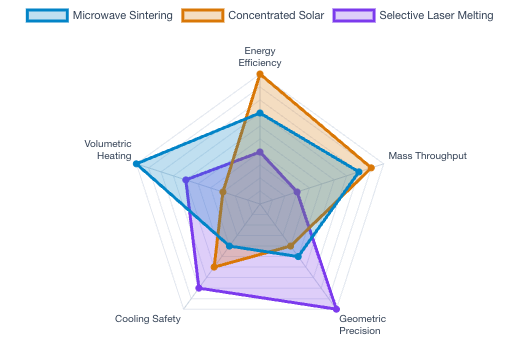
\includegraphics[width=0.75\textwidth]{figures/fig2_sintering_radar.png}
    \caption{\textbf{Multi-attribute engineering trade-off comparison of lunar regolith sintering modalities.} Normalized performance radar chart (scale 1--10) comparing Microwave Sintering ($2.45/5.8\,\mathrm{GHz}$), Concentrated Solar Sintering (ALM), and Selective Laser Melting (SLM) across energy efficiency, mass throughput, geometric precision, thermal stress safety, and volumetric heating capability.}
    \label{fig:sintering_radar}
\end{figure}

\begin{table}[t!]
\small
\centering
\caption{\textbf{Key operational and technological parameters of lunar regolith additive manufacturing modalities for bio-infrastructure.}}
\label{tab:manufacturing_modalities}
\begin{tabularx}{\textwidth}{lXXXXX}
\toprule
\textbf{Modality} & \textbf{Heating Mechanism} & \textbf{Operating Temp.} & \textbf{Specific Power Footprint} & \textbf{Geometric Resolution} & \textbf{Primary BLSS Application} \\
\midrule
Microwave Sintering ($2.45/5.8\,\mathrm{GHz}$) & Volumetric dielectric loss coupling with $\mathrm{npFe}^0$ and ilmenite\cite{taylor2005microwave,xi2026multiphysics,chen2024measurement} & $1050^\circ\mathrm{C}\text{--}1200^\circ\mathrm{C}$\cite{ming1989lunar} & Electrical (Magnetron/Solid-State); $\sim 1.2\,\mathrm{kWh/kg}$\cite{ming1989lunar} & Moderate ($1\text{--}5\,\mathrm{mm}$ feature size)\cite{taylor2005microwave,xi2026multiphysics} & Volumetric growth blocks, filter media, structural pavers\cite{ming1989lunar,metzger2023cost} \\
\addlinespace
Concentrated Solar Sintering (ALM) & Concentrated radiative flux and surface thermal conduction\cite{ming1989lunar,fateri2019solar,meurisse2018regolight} & $1100^\circ\mathrm{C}\text{--}>1400^\circ\mathrm{C}$\cite{ming1989lunar} & Direct solar; zero electrical draw during lunar day\cite{ming1989lunar} & Coarse-to-Moderate ($2\text{--}10\,\mathrm{mm}$ layer)\cite{fateri2019solar,fateri2018additive} & Hydroponic troughs, drainage gutters, perimeter shielding\cite{ming1989lunar} \\
\addlinespace
Selective Laser Melting (SLM/SLS) & Focused optical absorption, local melt pool fusion\cite{ming1989lunar,goulas2017process} & $1200^\circ\mathrm{C}\text{--}1500^\circ\mathrm{C}$\cite{ming1989lunar} & High electrical draw; laser diodes ($\sim 3.5\,\mathrm{kWh/kg}$)\cite{ming1989lunar} & High ($50\text{--}200\,\mu\mathrm{m}$ resolution)\cite{ming1989lunar,goulas2017process} & Aeration nozzles, porous wicking pins, fluid manifolds\cite{ming1989lunar,goulas2017process,balla2021selective} \\
\bottomrule
\end{tabularx}
\end{table}
